% The lower bound at general margin: what is missing, what is not.

\section{Toward the matching lower bound}\label{sec:lower}

Krauth and M\'ezard conjectured the value of the limiting ratio
$M_N(\kappa)/N$ for every margin, not only at
$\kappa=0$~\cite{krauth1989storage}; the constant $0.833$ is the
zero-margin point of the conjectured curve $\alpha_\star(\kappa)$.
At $\kappa=0$ the conjecture is resolved: Ding and
Sun~\cite{ding2019capacity} proved $\alpha_\star$ is a lower bound
with positive probability, the sharp-threshold sequence of Nakajima
and Sun~\cite{nakajimasun2022} upgrades positive probability to
convergence in probability, Huang~\cite{huang2024capacity} proved the
matching upper bound, and the numerical hypotheses of both proofs are
certified~\cite{shmalo2026capacity}.  Away from $\kappa=0$ the upper
half is Theorem~\ref{thm:main}; the lower half has, at present, no
analytic theorem to certify.  This section delimits the gap: a lemma
on why unconditioned moment methods cannot close it at nonnegative
margins, an embedded bound that does give nonzero-margin capacity
lower bounds on the negative side, and a numerical verification that
the $\kappa$-dependent inputs of the Ding--Sun program hold at all
five certified margins.

\subsection{Plain second moments fail at every margin}

Write $Z=Z_{N,\kappa}$ for the number of $w\in\{-1,+1\}^N$ satisfying
all $M=\lceil\alpha N\rceil$ constraints, and
$q_\rho(\kappa)=\Prob(X\ge\kappa,\,Y\ge\kappa)$ for $(X,Y)$ bivariate
standard Gaussian with correlation $\rho$.

\begin{lemma}\label{lem:secondmoment}
For every $\kappa\in\R$ and $\alpha>0$,
\[
\liminf_{N\to\infty}\frac1N\log\frac{\E[Z^2]}{(\E Z)^2}
\;\ge\; c(\alpha,\kappa)\;>\;0 .
\]
Consequently the Paley--Zygmund bound applied to $Z$ gives only
$\Prob(Z>0)\ge e^{-cN+o(N)}$, and no bound depending on $\E Z$ and
$\E[Z^2]$ alone can do better, since a distribution placing mass
$(\E Z)^2/\E[Z^2]$ at $\E[Z^2]/\E Z$ and the rest at zero matches
both moments.  For $\kappa\ge0$ the same conclusion holds for every
weighted count $Z_f=\sum_w\prod_a f(\langle g_a,w\rangle/\sqrt N)$
with $f\ge0$ supported on $[\kappa,\infty)$ and
$0<\int f\,d\Phi<\infty$.
\end{lemma}

\begin{proof}
$\E Z=2^N\Psi(\kappa)^M$ by independence over constraints.  For a
pair $w,w'$ at overlap $\rho$ the constraint fields are bivariate
Gaussian with correlation $\rho$, so counting ordered pairs by
Hamming distance $k$,
\[
\E[Z^2]=2^N\sum_{k=0}^N\binom Nk\,q_{1-2k/N}(\kappa)^M .
\]
Fix $\rho_0\in(0,1)$, let $k^*=\lceil N(1-\rho_0)/2\rceil$ and
$\rho^*=1-2k^*/N$.  Keeping the single term $k^*$ and using
$\binom Nk\ge e^{N H(k/N)}/(N+1)$ with $H$ the natural-log binary
entropy ($H(p)=H(1-p)$, so the exponent may be written with
$(1+\rho_0)/2$),
\[
\frac1N\log\frac{\E[Z^2]}{(\E Z)^2}
\ge\underbrace{H\Bigl(\tfrac{1+\rho_0}2\Bigr)-\log2
+\alpha\bigl[\log q_{\rho_0}(\kappa)-2\log\Psi(\kappa)\bigr]}
_{=:\,\psi_{\alpha,\kappa}(\rho_0)}\;+\;O(N^{-1}\log N),
\]
the error, of order $N^{-1}\log N$, collecting the binomial
prefactor, the $|\rho^*-\rho_0|\le
2/N$ continuity of $\rho\mapsto\log q_\rho$ (differentiable, below),
and $|M-\alpha N|\le1$.  Now $q_0=\Psi(\kappa)^2$ and $H(1/2)=\log2$
give $\psi_{\alpha,\kappa}(0)=0$.  Reflecting the orthant to a joint
CDF, $q_\rho(\kappa)=\Phi_2(-\kappa,-\kappa;\rho)$, and Plackett's
identity $\partial\Phi_2/\partial\rho=\varphi_2$ with the symmetry
$\varphi_2(-\kappa,-\kappa;\rho)=\varphi_2(\kappa,\kappa;\rho)$ give
$\partial q_\rho/\partial\rho=\varphi_2(\kappa,\kappa;\rho)$ on
$(-1,1)$; at $\rho=0$ this is $\varphi(\kappa)^2$.  Since
$\frac{d}{d\rho}H(\tfrac{1+\rho}2)=\tfrac12\log\tfrac{1-\rho}{1+\rho}$
vanishes at $0$,
\[
\psi_{\alpha,\kappa}'(0)=\alpha\,
\frac{\varphi(\kappa)^2}{\Psi(\kappa)^2}\;>\;0 ,
\]
so $\psi_{\alpha,\kappa}(\rho_0)\ge\rho_0\,\psi'(0)/2>0$ for all
small $\rho_0>0$; fix such a $\rho_0$ and set
$c=\psi_{\alpha,\kappa}(\rho_0)$.  For the weighted counts, the diagonal
term of $\E[Z_f^2]$ is $2^N\E[f(X)^2]^M$, so either
$\E[Z_f^2]=\infty$ and the claim is trivial, or $f\in L^2(\Phi)$ and
Mehler's expansion gives
$\E[f(X)f(Y)]=\sum_{j\ge0}\rho^j\langle f,\mathrm{He}_j\rangle^2/j!$,
whose $\rho$-derivative at $0$ is $(\int xf\varphi\,dx)^2$; for
$f\ge0$ supported on $[\kappa,\infty)$ with $\kappa\ge0$ the
integrand $xf(x)\varphi(x)$ is nonnegative, and it vanishes almost
everywhere only if $f$ vanishes almost everywhere off the origin,
which $0<\int f\,d\Phi$ excludes; the argument
then runs unchanged.
\end{proof}

The mechanism is the asymmetry: pairs of solutions at small positive
overlap are exponentially favored over independent pairs at every
margin, which is what the AMP-conditioned second moment
of~\cite{ding2019capacity} is built to circumvent at $\kappa=0$, and
what any lower-bound proof must circumvent at every other margin.
The zero-margin instance of this failure is classical
(see the introduction of~\cite{ding2019capacity}); the content here
is the uniform mechanism and the closure over nonnegative-margin
weights.  For $\kappa<0$ the weighted closure genuinely fails, and
profitably so: a window weight symmetric about the origin has zero
linear Mehler coefficient, which is the next observation.

\subsection{A capacity lower bound at negative margins}

\begin{prop}\label{prop:embedded}
Let $\kappa<0$ and let $\alpha^{\mathrm{sym}}_c(K)=
\log2/(-\log\Prob(|X|\le K))$ denote the symmetric binary perceptron
threshold at width $K$.  For every
$\alpha<\alpha^{\mathrm{sym}}_c(|\kappa|)$, with probability
$1-o(1)$ the margin-$\kappa$ perceptron admits a solution:
$M_N(\kappa)/N\ge\alpha$ whp.
\end{prop}

\begin{proof}
If $|\langle g_a,w\rangle|/\sqrt N\le-\kappa$ for all $a$ then in
particular $\langle g_a,w\rangle/\sqrt N\ge\kappa$, so the symmetric
solution set at width $|\kappa|$ embeds in the margin-$\kappa$
solution set.  The symmetric threshold is
$\alpha^{\mathrm{sym}}_c$~\cite{aubin2019storage}; for Gaussian
disorder the satisfiability side below it holds with high
probability by Altschuler's critical-window
theorem~\cite{altschuler2022}.  (The lognormal limit of Abbe, Li,
and Sly~\cite{abbelisly2021} is proved for Rademacher disorder, and
Perkins and Xu~\cite{perkinsxu2021} treat the Gaussian case under a
single-critical-point hypothesis, so neither alone covers the model
here.)
\end{proof}

The bound is far from sharp --- at $\kappa=-0.05$ it gives
$0.215$ against the predicted $0.889$, at $\kappa=-0.45$ it gives
$0.655$ against $1.558$ --- but it is, as far as we know, the only
rigorous nonzero-margin lower bound presently available for the
one-sided Ising perceptron, and it is strictly positive on the whole
negative axis.

\subsection{The Ding--Sun condition at general margin}

The construction underlying the $\kappa=0$ lower bound
of~\cite{ding2019capacity} is written at general margin throughout
their Section~2: their equations (34)--(48) define, for parameters
$(\kappa_{\mathrm{all}},\alpha_{\mathrm{all}})$, an explicit
univariate function $S_{\kappa,\alpha}(\lambda)$ on
$[\lambda_{\min},1]$ built from the fixed point $(q_\star,\psi_\star)$
--- an entropy term through the two-spin measure $P_{H,D}$, a
constraint term through the conditional Mills law
$\varphi_\xi$, and a convex $\inf_s$ correction --- and their
Condition~1.2 is the statement $S_{0,\alpha_\star}(\lambda)<0$ for
$\lambda\notin\{0,1\}$.  The $\kappa$-analog of that hypothesis is
therefore already defined in their own notation, and every
$\kappa$-dependent ingredient it consumes is an object this paper
certifies: the fixed point, its uniqueness rectangle, and the
crossing (Theorem~\ref{thm:strip} and the deep enclosures of
Theorem~\ref{thm:main}).

We evaluated $S_{\kappa,\alpha_\star(\kappa)}$ in floating point
(the driver \texttt{ds\_condition.py} uses Gauss--Hermite and
conditional Gauss--Legendre quadrature) at the five certified margins
and at $\kappa=0$, checking the six endpoint identities
$H(0)=P(0)=A(0)=0$, $H(1)=-H_\star$, $P(1)=-P_\star$,
and $G_\star=H_\star+P_\star\approx0$ (with $H_\star$, $P_\star$ the
entropy and constraint halves of the free energy), and that the
conditional-mean check resolves at $10^{-12}$ or better at every
margin, as implementation controls.  The result is uniform
(Figure~\ref{fig:dscondition}): at every margin the curve is
strictly negative off $\{0,1\}$, at most
$-5\cdot10^{-5}$ outside windows of half-width $0.02$ around the two
roots (inside them it climbs to its maxima at the roots, reaching
$-1.6\cdot10^{-6}$ at the closest grid points), the maximum at
$\lambda=0$ is degenerate exactly as
at $\kappa=0$, and the whole family collapses nearly onto a single
shape, with $\lambda_{\min}$ drifting from $-0.441$ at
$\kappa=-0.45$ to $-0.421$ at $\kappa=0.13$.  These are diagnostics,
not certificates; certifying $S_{\kappa,\alpha_\star}<0$ off the
roots is a univariate problem of exactly the species the
Condition~\ref{cond:2var} machinery already handles, and we expect it
to be far easier than the two-variable certification carried out
here.

\begin{figure}[t]
\centering
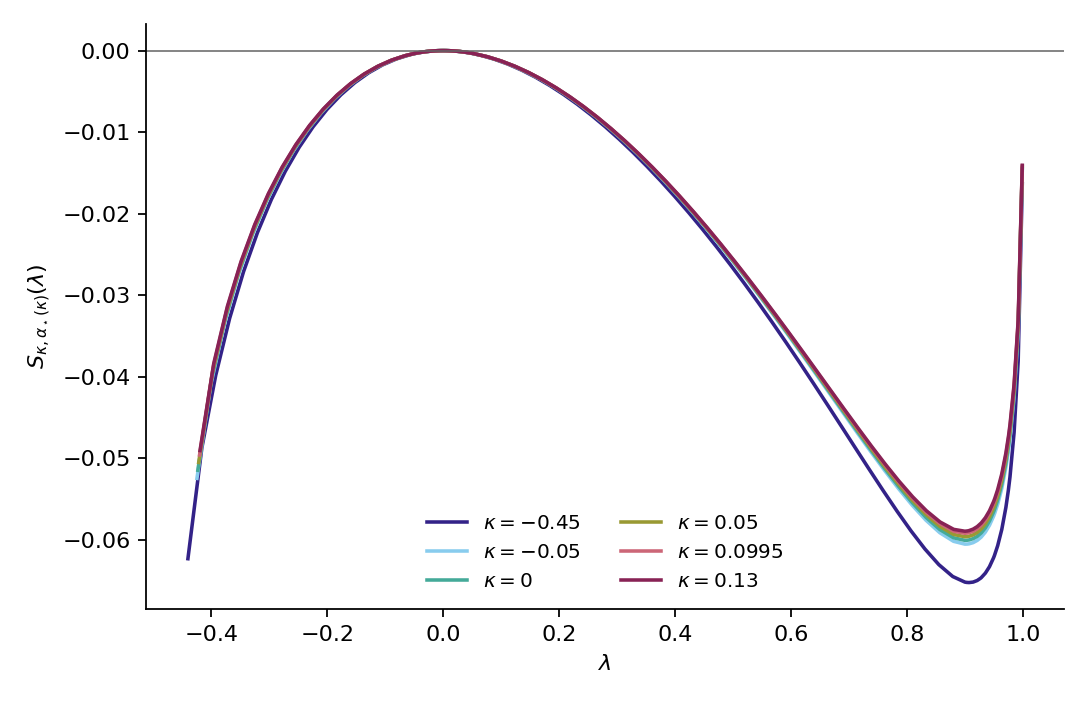
\includegraphics[width=0.85\linewidth]{ds_condition.png}
\caption{The general-margin Ding--Sun lower-bound condition,
evaluated at the five certified margins and $\kappa=0$: the
univariate function $S_{\kappa,\alpha_\star(\kappa)}$ of their
equation (48), whose nonpositivity off $\{0,1\}$ is the numerical
hypothesis of their second-moment argument.  All six curves are
negative off the two roots and nearly coincide.}
\label{fig:dscondition}
\end{figure}

What separates these verified inputs from a general-margin lower
bound is the probabilistic body of~\cite{ding2019capacity}: the
AMP-conditioned moment computation of their Sections~2--7, whose
displays carry $\kappa_{\mathrm{all}}$ explicitly but whose proofs
are executed at $\kappa=0$.  An audit of that body would need, beyond
the certified inputs above: a priori bounds at margin (the upper one
is free at every $\kappa$ from the first moment, since
$\E Z\to0$ exponentially above the annealed threshold
$-\log2/\log\Psi(\kappa)$; the lower one is
Proposition~\ref{prop:embedded} for $\kappa<0$ and open for
$\kappa>0$), the state-evolution inputs (generic in the
nonlinearity, hence in $\kappa$), and the sharp-threshold transfer
of~\cite{nakajimasun2022} if convergence in probability rather than
positive probability is wanted.  We record this as the concrete
route to the exact threshold at the certified margins: the numerical
side is done at six points and the analytic side is a
$\kappa$-generalization audit of an existing proof, not a new
construction.
